%!TEX root = geometry.tex
\stepcounter{lecture}
\setcounter{lecture}{5}
\sektion{Hyperbolic geometry}

\subsection{Hyperboloid model} % (fold)
\label{sub:hyperboloid_model}

\begin{definition}
	We consider the surface $S \subset \R^3$ given by $x^2+y^2-z^2=-1$, $z<0$. This \emph{hyperboloid sheet} gives us another way to think of points. The sketch below illustrates the sheet: it asymptotically approaches the planes $x=y$, $y=z$ and $z=x$; we take a cross section view.

	\begin{center} % Geo 11/1 
		\begin{tikzpicture}[yscale=1.4, rotate=180]
			\bigarrow (2,0) -- (-2,0);
			\bigarrow (0,2.5) -- (0,-1);

			\begin{scope} [yscale=3, xscale=1.4]
				\draw [thick] (0,0.3) arc (-90:-55:1.8);
			\end{scope}

			\begin{scope} [yscale=3, rotate=180, xscale=1.4]
				\draw [thick] (0,-0.3) arc (90:55:1.8);
			\end{scope}

			\draw [thick] (-0.05,0.9) -- (0.05,0.9);

			\draw [dashed] (2,2) -- (0,0) -- (-2,2);
		\end{tikzpicture}
	\end{center}

	With this in mind, we give $\R^3$ the \emph{Minkowski metric}
	\begin{equation*}
		g^M = \dif{x^2} + \dif{y^2} - \dif{z^2}.
	\end{equation*}
	Formally, we've taken the surface $x^2+y^2+z^2=-1$, and replaced $z$ by $iz$.
\end{definition}

At first, these two definitions might seem unnatural, but in some sense, it's the most natural thing in the world. Note, however, that the Minkowski metric is \emph{not} a Riemannian metric. It is sometimes called the \emph{pseudo-Riemannian metric}.

As before, we consider the stereographic projection $\pi:S\to\C$. And as before, we have a ``north pole'' $\NN=(0,0,1)$, and for any $\pi\in S$ that is not $\NN$, we define $\pi(\pp)$ to be the intersection of $NP$ with the $xy$ plane. Thus
\begin{equation*}
	\pi\left( (x,y,z) \right) = \f{x+iy}{1-z} = w,
\end{equation*}
the same as the sphere. Inversion is similar; we first consider
\begin{equation*}
	\left\vert w \right\vert^2
	= \f{x^2+y^2}{\left( 1-z \right)^2}
	= \f{z^2-1}{\left( 1-z \right)^2}
	= \f{z+1}{z-1}
	\implies
	z = \f{\left\vert w \right\vert^2+1}{\left\vert w \right\vert^2-1}.
\end{equation*}
Now, if $z<0$, then $\left\vert w \right\vert^2<1$, and so
\begin{equation*}
	\Image(\pi) = D = \left\{w\iC: \left\vert w \right\vert<1\right\}.
\end{equation*}
So using the same process as the sphere, we have
\begin{equation*}
	1-z = \f{2}{1-\left\vert w \right\vert^2},
\end{equation*}
and so the inverse is given by
\begin{equation*}
	\pi^{-1}(w) = \left( \f{2\,\Re(w)}{1-\left\vert w \right\vert^2}, \f{2\,\Im(w)}{1-\left\vert w \right\vert^2}, \f{\left\vert w \right\vert^2+1}{\left\vert w \right\vert^2-1} \right).
\end{equation*}

% subsection hyperboloid_model (end)

\subsection{Unit disc model} % (fold)
\label{sub:unit_disc_model}

Let $g^D$ be the metric induced on $g$ using $g^M$, that is,
\begin{equation*}
	g^D = \dif{\sigma_1^2} + \dif{\sigma_2^2} - \dif{\sigma_3^2},
\end{equation*}
where
\begin{equation*}
	\sigma(x,y) = \left( \f{2x}{1-x^2-y^2}, \f{2y}{1-x^2-y^2}, \f{1+x^2+y^2}{1-x^2-y^2} \right).
\end{equation*}
Note that we've now switched to using $x$ and $y$ as coordinates on $D$, not on $\R^3$. This is essentially the same calculation as for $g^{S^2}$, and we obtain
\begin{equation*}
	g^D = \f{4\left( \dif{x^2} + \dif{y^2} \right)}{(1-x^2-y^2)^2}.
\end{equation*}
Again, this is conformal to $g^E$.

% subsection unit_disc_model (end)

\subsection{Upper half-plane model} % (fold)
\label{sub:upper_half_plane_model}

This gives us another way to do hyperbolic geometry. Let $H=\{z\iC: \Im(z)>0\}$, the upper half-plane. Define
\begin{equation*}
	\fullfunction{\varphi}{\C_\infty}{\C_\infty}{z}{(z-i)/(z+i)}
\end{equation*}
We saw in section~\ref{sec:m_bius_transformations} that $\phi(\R\cup\{\infty\}) = S^1$, and since $\phi(i)=0$, we have $\phi(H)=D$.

\begin{definition}
	Let $g^H$ be the Riemannian metric on $H$ induced from $g^D$ using $\phi$:
	\begin{equation*}
		g_\pp^H(\va,\vb) = g^D_{\phi(\pp)}(\ddif{\phi}{\pp}(\va), \ddif{\phi}{\pp}(\vb))
	\end{equation*}
	By definition, $\phi$ is a Riemann isometry from $g^H$ to $g^D$.
\end{definition}

To compute $g^H$, write $w=x+iy$. Then $\dif{x^2} \dif{y^2} = \dif{w} \dif{\wbar}$. For $w\in D$, we have
\begin{equation*}
	w=\phi(z) = \f{z-i}{z+i} = 1-\f{zi}{z+i}.
\end{equation*}
By careful consideration, this gives us
\begin{equation*}
	\dif{w} = \f{zi}{\left( z+i \right)^2} \qqand
	\dif{\wbar} = \f{-zi}{\left( \zbar-i \right)^2} \dif{\zbar}.
\end{equation*}
By substituting appropriately, and writing $z=u+iv$, we have
\begin{align*}
	g^H
	= \f{4\left( \df{zi \dif{z}}{\left( z+i \right)^2} \right) \left( \df{-zi \dif{\zbar}}{\left( \zbar-i \right)^2} \right)}{\left( 1-\df{\left( z-i \right)\left( \zbar+i \right)}{\left( z+i \right)\left( \zbar-i \right)} \right)^2}
	&= \f{16 \dif{z} \dif{\zbar}}{\left[ \left( z+i \right)\left( \zbar-i \right) - \left( z-i \right)\left( \zbar+i \right) \right]^2} \\
	&= \f{16 \dif{z} \dif{\zbar}}{\left[ zi\left( \zbar-z \right) \right]^2} \\
	&= \f{16 \dif{z} \dif{\zbar}}{\left( 4v \right)^2} \\
	&= \f{\dif{u^2} + \dif{v^2}}{v^2}.
\end{align*}

% $G^H = \PSL_2(\R)$ acts on $H$ $\leftrightarrow$ $G^D = {\phi: \phi(z) = e^{i\theta} \f{z-a}{az-1}, \theta\iR, a\in D}$
% $G^D = \phi G^H \phi^{-1}$.

% subsection upper_half_plane_model (end)

\subsection{Geometry of the hyperbolic plane} % (fold)
\label{sub:geometry_of_the_hyperbolic_plane}

\lecturemarker{12}{27 Feb}
We've now seen two models of the hyperbolic plane: the upper half-plane model $H$, and the unit disc model $D$.

In particular, recall that $G^H = \PSL_2(\R)$ acts on $H$, with
\begin{equation*}
	G^D = \left\{\phi: \phi(z) = e^{i\theta} \f{z-a}{az-a}, \theta\iR, a\in D\right\} = \phi G^H \phi^{-1}.
\end{equation*}
This $\phi$ gives us a way to compare boundaries: $\boundary{H} = \R\cup\infty=\R_\infty$, and $\boundary{D} =S^{\,1}$. Then $\phi(\R_\infty) = S^{\,1}$.

We may use both of these models, depending on which is more convenient at the time. We use $\HH$ to denote either one, without specifying which. With these two models in hand, we can discuss all the features of geometry that we've talked about before.

Angles are simple. Both $g^D$ and $g^H$ are conformal, so angles between curves in $g^D$ or $g^H$ is the same as the Euclidean angle.

Now let's consider isometries. Let $\Isom(H)$ be the group of Riemannian isometries of $(H,g^H)$, and similarly, $\Isom(D)$ be the group of Riemannian isometries of $(D,g^D)$. We come to our first result:

\begin{proposition}
	$G^H \subset \Isom(H)$.
\end{proposition}

\vspace{-8pt}

Note that $G^H$ isn't all isometries, as not all isometries are orientiation preserving.

\begin{proof}
	Recall that $G^H = \PSL_2(\R)$ is generated by three kinds of maps:
	\begin{enumerate}
		\shortskip
		\item $z\mapsto z+b$, $b\iR$;
		\item $z \mapsto az$, $a\iR$;
		\item $z\mapsto -1/z$.
	\end{enumerate}
	It suffices to check that (i), (ii) and (iii) are in $\Isom(H)$.
	\begin{enumerate}
		\item If $z=\phi(z\p) = z\p+b$, then we have
		\begin{equation*}
			\begin{array}{lcl}
				x=x\p + b & & \dif{x} = \dif{x\p} \\
				y=y\p & & \dif{y} = \dif{y\p}.
			\end{array}
		\end{equation*}
		Thus we have
		\begin{equation*}
			g^H
			= \f{\dif{x^2} + \dif{y^2}}{y^2}
			\xrightarrow[\text{induced by $\phi$}]{\text{metric}}
			\f{\left( \dif{x\p} \right)^2 + \left( \dif{y\p} \right)^2}{\left( y\p \right)^2}
			= g^H.
		\end{equation*}

		\item If $z=\phi(z\p)=az\p$, then $x=ax\p$, $y=ay\p$ and
		\begin{equation*}
			g^H
			= \f{\dif{x^2} + \dif{y^2}}{y^2}
			\longrightarrow
			\f{a^2\left( \dif{x\p} \right)^2 + a^2\left( \dif{y\p} \right)^2}{a^2\left( y\p \right)^2} = g^H.
		\end{equation*}

		\item If $z=\phi(w)=-1/w$, then
		\begin{equation*}
			\dif{z} = \f{\dif{w}}{w^2} \qqand
			\dif{\zbar} = \f{\dif{\wbar}}{\wbar^2}.
		\end{equation*}
		Then we have
		\begin{equation*}
			g^H
			= \f{\dif{x^2} + \dif{y^2}}{y^2}
			= \f{\dif z \dif{\zbar}}{\left( \f{1}{2}\left( \zbar-z \right) \right)^2}
			\longrightarrow
			\f{\left( -\f{\dif{w}}{w^2} \right)\left( -\f{\dif{\wbar}}{\wbar^2} \right)}{\left( \f{1}{2}\left( \f{1}{\wbar}-\f{1}{w} \right) \right)^2}
			= \f{\dif{w} \dif{\wbar}}{\left( \f{1}{2}\left( w-\wbar \right) \right)^2} = g^H. \qedhere
		\end{equation*}
	\end{enumerate}
\end{proof}

\begin{corollary}
	$G^D \subset \Isom(D)$
\end{corollary}

\begin{proof}
	If $\psi \in G^D$, then $\psi=\phi_0 \chi \phi_0^{-1}$, where $\chi\in G^H$. Thus $\phi_0, \chi, \phi_0^{-1}$ are all isometries, and the composition of isometries is an isometry. Thus $\psi \in \Isom(D)$.
\end{proof}

Now we consider hyperbolic lines. These are defined in a very similar way to spherical lines.

\begin{definition}
	A \emph{hyperbolic line} in $H$ is $L = H \cap C$, where $C$ is a Euclidean line or circle which is perpendicular to $\partial{H}$. A similar definition under the disc model comes by replacing $H$ by $D$.

	\begin{center}
		\begin{minipage}{0.4\textwidth} % Geo 12/1, 12/1b
		\centering
		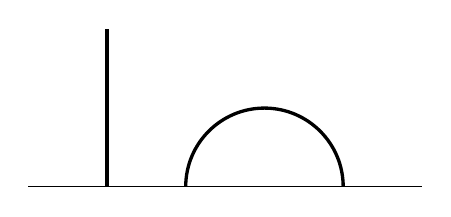
\begin{tikzpicture}
			\draw (0,0) -- (5,0);
			\draw [very thick] (1,0) -- (1,2);
			\draw [very thick] (4,0) arc (0:180:1);
		\end{tikzpicture}
	\end{minipage}
	\hspace{0.2cm}
	\begin{minipage}{0.4\textwidth}
		\centering
		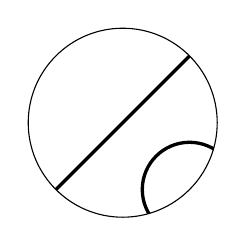
\begin{tikzpicture}[scale=0.6]
			\draw (2,2) circle (2);
			\clip (2,2) circle (2);
			\draw [very thick] (2,2) -- ++ (45:2) -- ++ (-135:4);
			\draw [very thick] (2,2) ++ (-45:2) circle (1);
		\end{tikzpicture}
	\end{minipage}

	\begin{minipage}{0.4\textwidth}
		\centering
		half-plane model
	\end{minipage}
	\hspace{0.2cm}
	\begin{minipage}{0.4\textwidth}
		\centering
		disc model
	\end{minipage}
	\end{center}
\end{definition}

For the rest of the chapter, when we say ``line'', we mean ``hyperbolic line'' unless otherwise specified.

Once we have lines, then it's natural to define rays:

\begin{definition}
	If $\gamma:\R\to H$ is a parameterisation of a line, then $R=\gamma([c,\infty))$ is a \emph{hyperbolic ray} starting at $\gamma(c)$ and with direction $\gamma\p(c)$.
\end{definition}

Now let's consider a few basic results involving lines:

\begin{lemma}
	$L$ is a line in $H$ if and only if $\phi_0(L)$ is a line in $D$.
\end{lemma}

\begin{proof}
	As $\phi_0\in\Mobgp$, it preserves angles, and it takes Euclidean lines and circles to Euclidean lines and circles. Also, $\phi_0(\boundary{H}) = \boundary{D}$. Thus, if $L$ is a line in $H$, then $\phi_0(L)$ is a line in $D$.

	The converse is similar.
\end{proof}

\begin{lemma}
	Given $\va \neq \vec{0}$, there is a unique hyperbolic line through $\vec{0} \in D$ which is tangent to $\va$ at $\vec{0}$.
\end{lemma}

\begin{proof}
	First we show that any line through $\vec{0}$ is a diameter of $D$. Suppose $C$ is a Euclidean circle passing through $\vec{0}$, perpendicular to $\boundary{D}$. Let $B$ be its centre.

	% \begin{center} % Geo 12/3
	% 	\begin{tikzpicture}
	% 		\draw [thick, red] (0,0) circle (1.4);
	% 		\draw [thick, blue] (2,0) circle (2);
	% 		\draw (0,0) node [below left] {$O$} -- (2,0) node [below right] {$B$} -- (0.49,1.31) -- cycle;
	% 		\draw (0.42,1.31) node [above=2pt] {$A$};

	% 		\foreach \s/\t in {0/0, 2/0, .49/1.31} {\draw (\s,\t) node {$\bullet$};}
	% 	\end{tikzpicture}
	% \end{center}

	Let $A$ be a point in $C \cap \boundary{D}$, then $\triangle OAB$ is isoceles. Thus $\angle OAB = \pi/2 = \angle AOB$, and so the sum of the angles is more than $\pi$. But this is ridiculous.

	The lemma now follows, sine there's a unique Euclidean line through $\vec{0}$ with direction vector $\va$.
\end{proof}

\begin{corollary}
	If $p\in\HH$ and $\va\neq 0$, then there's a unique ray stating at $\pp$ with direction vector $\va$.
\end{corollary}

\begin{proof*}
	[In $D$] Choose $\psi \in G^D$ with $\psi(\pp)=0$, such as $\psi(z) = \df{z-p}{\overline{p}z-1}$.

	Then there's a unique ray $R\p$ starting at $\vec{0}$ with direction $\dif{\psi_p(\va)} \neq 0$. Then the ray $R$ which we want is $R=\psi^{-1}(R\p)$. \qed
\end{proof*}

\begin{proposition}
	If $R_1,R_2$ are hyperbolic rays starting at $p_1,p_2 \iH$, then there is $\psi\in G$ with $\psi(p_1) = p_2$, $\psi(R_1)=R_2$.
\end{proposition}

\begin{proof*}
	[In $D$] Let $R_0$ be the positive real axis. Let
	\begin{equation*}
		\psi_1(z) = \f{z-p_1}{\overline{p_1}z-1}.
	\end{equation*}
	If $\psi_1(p_1)=0$, then $\psi_1(R_1)$ is a radius of $D$.
	\begin{center}
		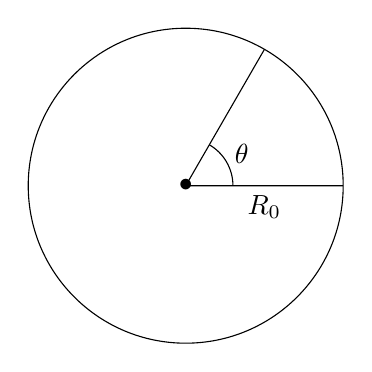
\begin{tikzpicture}[scale=2]
			\draw (0,0) circle (1) node {$\bullet$};

			\draw (1,0) -- (0,0) -- ++ (60:1);
			\draw (0.3,0) arc (0:60:0.3);
			\draw (0.25,0.2) node [right] {$\theta$};

			\draw (0.5,0) node [below] {$R_0$};
		\end{tikzpicture}
	\end{center}

	Let $\psi_R(z) = e^{-i\theta} \psi_1(z)$, where $\theta$ is the angle between $R_0$ and $\psi_1(R_1)$. Then $\psi_{R_1}(R_1) = R_0$. Construct $R_2$ similarly, and then take $\psi = \psi_{R_2}^{-1} \circ \psi_{R_1}$. \'.e'
\end{proof*}

\begin{proposition}
	There's a unique line containing two distinct points $p_1,p_2 \iH$.
\end{proposition}

\begin{proof*}
	[In $D$] Choose $\psi \in G^D$ with $\psi(p_1) = \vec{0}$. There's a unique hyperbolic line $L$ containing $\vec{0}$ and $\psi(p_2)$, namely through the diameter of $D$ through $\psi(\overline{p_2})$. Thus $\psi^{-1}(L)$ is the unique line containing $p_1$ and $p_2$. \qed
\end{proof*}

\begin{proposition}
	Two lines $L_1$ and $L_2$ intersect in at most one point in $\HH$.
\end{proposition}

\begin{proof*}
	[In $H$] After applying an element $\psi\in G^H$, we may assume that
	\begin{itemize}
		\shortskip
		\item $\psi(L_1)$ is the positive imaginary axis.
		\item $\psi(L_2)$ is (i) a circle centred on the real axis or (ii) a vertical line
	\end{itemize}
	Consider the two cases for $\psi(L_2)$:
	\begin{enumerate}
		\shortskip
		\item At most one intersection with $\psi(L_1)$ in $H$ (other is in the lower half-plane);
		\item Has none. \qed
	\end{enumerate}
\end{proof*}

This final proposition motivates the following definition:

\begin{definition}
	We say that $L_1$ and $L_2$ are \emph{haroparallel} if they intersect in $\boundary{\HH}$ and are \emph{ultraparallel} if they do not intersect in $\boundary{\HH}$.

	\begin{center}
		\begin{minipage}{0.4\textwidth} % Geo 12/5
		\centering
		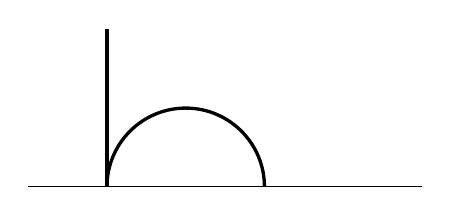
\begin{tikzpicture}
			\draw (0,0) -- (5,0);
			\draw [very thick] (1,0) -- (1,2);
			\draw [very thick] (3,0) arc (0:180:1);
		\end{tikzpicture}
	\end{minipage}
	\hspace{0.2cm}
		\begin{minipage}{0.4\textwidth}
		\centering
		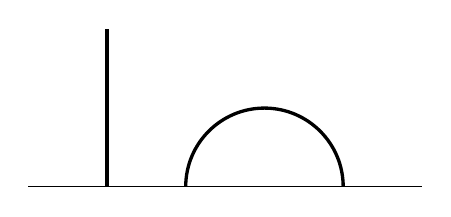
\begin{tikzpicture}
			\draw (0,0) -- (5,0);
			\draw [very thick] (1,0) -- (1,2);
			\draw [very thick] (4,0) arc (0:180:1);
		\end{tikzpicture}
	\end{minipage}

	\begin{minipage}{0.4\textwidth}
		\centering
		haroparallel
	\end{minipage}
	\hspace{0.2cm}
	\begin{minipage}{0.4\textwidth}
		\centering
		ultraparallel
	\end{minipage}
	\end{center}

	If $L$ is a line, $p\not\in L$, then there are infinitely many ultraparallel lines to $L$ that pass through $p$.
\end{definition}

	\pagebreak

Now we consider distance; specifically, the shortest distance between two points.

\begin{proposition}
	If $p,q\iH$, then the line segment from $\pp$ to $\qq$ is the shortest path from $\pp$ to $\qq$ in $H$.
\end{proposition}

\begin{proof*}
	[In $H$] Let $L$ be the unique line segment from $\pp$ to $\qq$. After composing with $\psi\in G$, we may assume that $L$ is the positive real axis.

	So we have $p=ia$, $q=ib$, $a,b\iR$.  Let $\gamma(t)$ be a path from $\pp$ to $\qq$ in $H$. Then
	\begin{equation*}
		L_{g^H}(\gamma)
		= \int_0^1 \sqrt{\f{\gamma_1^2+\gamma_2^2}{\gamma_2^2}} \dif{t}
		\geq \int_0^1 \left\vert \f{\gamma_2\p(t)}{\gamma_2\p(t)} \right\vert \dif{t}
		\geq \left\vert \int_0^1 \f{\gamma\p(t)}{\gamma(t)} \dif{t} \right\vert
		= \left\vert \ln b - \ln a \right\vert
		= \left\vert \ln(b/a) \right\vert.
	\end{equation*}
	with equality if and only if $\gamma_1\p=0$ and $\gamma_2\p$ has constant sign; that is, if $\gamma$ is a vertical line segment. \qed
\end{proof*}

\begin{corollary}
	The distance from $ia$ to $ib$ in $H$ is $\left\vert \ln(b/a) \right\vert$.
\end{corollary}

\begin{corollary}
	The distance from $\vec{0}$ to $re^{i\theta}$ in $D$ is $\ln\left[ (1+r)/(1-r) \right] = 2\tanh^{-1} r$.
\end{corollary}

% subsection geometry_of_the_hyperbolic_plane (end)

\subsection{Isometries of the hyperbolic plane} % (fold)
\label{sub:isometries_of_the_hyperbolic_plane}

\lecturemarker{13}{4 Mar}
We extend complex conjugation to a map $c:\C_\infty \to \C_\infty$ by setting $c(\infty) = \infty$. Now, if $\phi_A$ is the Möbius transformation defined by the matrix $A\in\GL_2(\C)$, then we see that
\begin{equation*}
	\phi_A \circ c = c \circ \phi_{\bar{A}}.
\end{equation*}

\begin{definition}
	The \emph{extended Möbius group} is given by
	\begin{equation*}
		\overline{\Mobgp} = \left\{ \phi:\C_\infty \to \C_\infty : \phi\in\Mobgp \text{or } \phi\circ c\in\Mobgp \right\}.
	\end{equation*}
\end{definition}

We observe that $c^2=\iota$, so the second condition is equivalent to saying that $\phi = \psi\circ c$, where $\psi\in\Mobgp$. It follows from our first equation that the extended Möbius group is closed under composition, and thus it indeed forms a group, containing the Möbius group as an index two subgroup.

Then elements of $\Mobgp$ are \emph{orientation preserving}, while elements of $\overline{\Mobgp}$ not in $\Mobgp$ are \emph{orientation reversing}. We can compare this to rotations and reflections in Euclidean geometry. We already have our rotations (given by Möbius maps), so now let's consider reflections:

\begin{definition}
	If $C\subset\C_\infty$ is a Euclidean line or circle, the reflection in $C$ is the extended Möbius transformation defined by
	\begin{equation*}
		R_C = \psi^{-1} \circ c \circ \psi,
	\end{equation*}
	where $\psi\in\Mobgp$ satisfies $\phi(C) = \R\cup\{\infty\}$.
\end{definition}

Hopefully this definition is reasonably intuitive; now we just need to check that it makes sense. We need to check that our choice of $\psi$ doesn't matter. So suppose we have $\psi\p(C)=\R\cup\{\infty\}$. Then $\psi\p \circ \psi^{-1}(\R) = \R$, and so $\psi\p \circ \psi^{-1} = \phi_A$, for some $A\in\GL_2(\R)$. (As in the Euclidean plane, two reflections form a rotation.) Then
\begin{equation*}
	\psi^{\,\prime^{-1}} \circ c \circ \psi\p
	= \psi^{-1} \circ \phi^{-1}_A \circ c \circ \phi_A \circ \psi
	= \psi^{-1} \circ c \circ \psi,
\end{equation*}
and so $R_C$ is well-defined.

\begin{example}
	If $C$ is the unit circle, then $R_C=\psi_0 \circ c \circ \psi_0^{-1}$, and so
	\begin{equation*}
		R_C(z)
		= \psi_0\left( -i\,\f{\zbar+1}{\zbar-1} \right)
		= \f{-i\f{\zbar+1}{\zbar-1} - i}{-i\f{\zbar+1}{\zbar-1} + i}
		= \f{1}{\zbar}.
	\end{equation*}
	More generally, if $C_r$ is a circle of radius $r$ centred at $0$, then $R_{C_r} = \psi_r \circ R_{C_1} \circ \psi_{1/r}$, where $\psi_a(z) = az$. Thus $R_{C_r} = r^2/\zbar$.
\end{example}

\begin{proposition}
	$\overline{\Mobgp}$ is generated by reflections.
\end{proposition}

\begin{proof}
	It is enough to check that the maps
	\begin{enumerate}
		\shortskip
		\item $z\mapsto z+b$, $b\iC$;
		\item $z\mapsto az$, $a\iC$, $a\neq 0$;
		\item $z\mapsto 1/z$;
	\end{enumerate}
	are compositions of reflections, since these maps generate $\Mobgp$.
	
	Map (i) is generated by $R_{L_1} \circ R_{L_2}$, where $L_1$ and $L_2$ are two Euclidean lines perpendicular to $b$ and separated by a distance $b/2$.

	For map (ii), multiplication by $a\iR$ is $R_{C_1} \circ R_{C_2}$, where $C_2$ is the unit circle and $C_1$ is a circle of radius $\sqrt{a}\,$ centred at the origin, while multiplication by $e^{i\theta}$ is $R_{L_1} \circ R_{L_2}$, where $L_1$ and $L_2$ are two lines which intersect in an angle $\theta/2$ at the origin. Using these two maps, we can compose for any $a\iC\backslash\{0\}$.

	Finally, map (iii) is the composition of reflection in the unit circle with reflection in $\R$. This completes the proof.
\end{proof}

We can view the groups $\Isom(S^2)$, $\Isom(\R^2)$ and $\Isom(D)$ as subgroups of the extended Möbius group, corresponding to the extension of the following subgroups of $\Mobgp$ by $c$:
\begin{align*}
	\Isom^+(S^2) &= \left\{\phi_A : A = \mat{\alpha & \beta \\ -\overline{\beta} & \overline{\alpha}}, \det A = 1 \right\}, \\
	\Isom^+(\R^2) &= \left\{\phi_A : A = \mat{\alpha & \beta \\ 0 & \overline{\alpha}}, \det A = 1 \right\}, \\
	\Isom^+(D) &= \left\{\phi_A : A = \mat{\alpha & \beta \\ \overline{\beta} & \overline{\alpha}}, \det A = 1 \right\}, \\
\end{align*}

% subsection isometries_of_the_hyperbolic_plane (end)